\section{Methodology}
	The approach I undertake in this study is similar to previous works in the field. Initially, data is gathered on a given theme. In the case of my research, the main query I wish to study would regard Tweets relating to the subject of E-Commerce platforms.
	\par
	On of the motives of this research is to observe whether information originating from social media can be evaluated in real-time. With this consideration in mind, the data should bear as much resemblance to a live information torrent on Tweeter as possible. Acknowledging this consideration, the raw data in gathered in the form of Tweets originating from the Twitter databases. I collect the data synchronously, as it is intercepted by the servers. The \textit{Streaming} Application Programming Interface (API)\cite{stream_api} is usually implemented in such use-cases. Using the \textit{Streaming} API, a connection is established to the servers, which captures a narrow stream (about 15\%) of all Tweets relevant to a given search term. 
	\par
	The captured data, must then be restructured to fit the data-model of this study, namely appropriate input for Machine Learning algorithms. This includes a preliminary analysis of the data and removal of incomplete observations. The data structure in which Tweets are stored allow for a dynamic non-standard structure, which in turn means they vary in properties. Therefore some Tweets must be adapted to conform to a unitary pattern. It is also quite common for Tweets to retrospectively be removed, either by themselves or by Twitter moderators. Such Tweets cannot be analyzed, since they are no longer available on-line. The process of gathering data and cleansing it is discussed in \hyperref[sec:collect_data]{Part [4.1]}.
	\par
	The next stage entails representing the data in a form which is suitable for Machine Learning Algorithms. For this purpose, I build \textit{features}\footnote{\label{ml_note}Machine Learning nomenclature} for each observation. \textit{Features} are unique properties of the data, which are used to describe it. Different types of \textit{Features} are used in accordance with the Learning approach undertaken. These approaches  we discuss in \hyperref[build_features]{Part [4.2]}.
	\par
	These features are then analyzed for consistency and correctness. Subsequently, the features are passed into different Machine Learning algorithms, in order to \textit{train}\footnotemark[1] them. \textit{Training} is the process of deducing the decision rules for classifying the data into one of the categories. This deduction is based on the information the algorithm draws from the input data. Afterwards, the empirical success of these different algorithms will be statistically measured the summarized. Additionally, implications are to be drawn about other use-cases, which are out of the scope of this research. 
	
	\subsection{Training Classifier}
	The purpose of \textit{training} is to create Classifiers, which automatically recognize and \textit{label} new observations. The intrinsic	decision algorithm, through which the Classifier will decide how to classify a novel observation, usually remain hidden and operate as a black-box of sorts. Since the decision rules could be numerous and far from intuitive for human readers. This is especially the case, when said algorithms are convolutional. Convolutional machine learning schemes, such as Deep Neural Networks, may incorporate numerous stages of parameter construction which renders them practically incomprehensible to human users. The actual implementation of all the algorithms would be programmed in the Python programming language and will be primarily making use of the scikit-learn\cite{scikit-learn} module.
	\par
	The data used for the purpose of this study consolidates 12.520 unique Tweets. For the purpose of reaching robust results, the \textit{Hold-out Method} is used as follows. For each instance of \textit{Algorithm training} the entire data corpus is split into two parts - a training set and testing set. The training set would usually be allocated the larger portion of the data (about 70\%) and would be used, as the name suggests for training the Classifiers. The rest of the data (about 30\%) would be used for testing the Classifiers accuracy. During each such training-testing session, the data corpus is shuffled. This in turn means, that the training and testing sets constantly differ. This process of splitting, training and testing using different data in each iteration should produce statistically significant results. This method of constantly splitting the data randomly ensures the results robustness.
	\par
	The following paragraphs expand on the different Machine Learning schemes. Figure 3 illustrates these schemes according to their types.
	
	\begin{figure}[h]
		
		\centering
		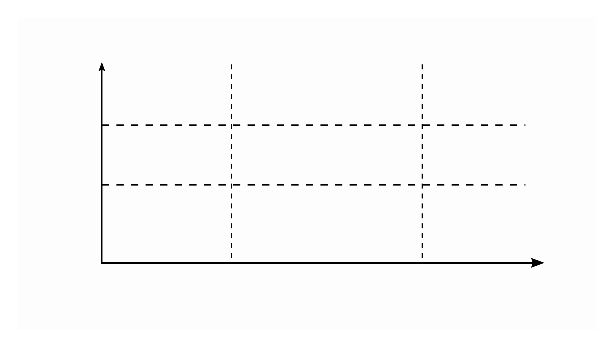
\includegraphics[width=0.5\textwidth]{methods}
		\caption{Clustering of Different Classifiers}
	\end{figure}
	
	\subsection{Supervised Learning}
	
	\subsubsection*{Regressions}
	One approach and probably the most basic one is simply running a regression with all the features as the independent variables and the a numeric representation of the classes as the dependent variable. Some threshold value for the classes must be determined since the estimate for the explained variable, will have a non-deterministic value.
	\par
	\paragraph{Linear Regression} 
	This method builds a linear dependency system between the explained variable (the \textit{Class} in this case) and the explaining variables (\textit{features}). With the \textit{Bag-of-Words} approach, each variable \textit{x} is a dummy variable indicating whether a given word \textit{m} is present in Tweet \textit{i}. The estimations parameters, which are denoted with $\beta_j$ are derived using Ordinary Least Squares. In itself, the linear regression estimation is a weak predictor for the purpose of classification, but it allows for calculating other useful statistics such as the coefficient of determination, commonly known as $R^2$. This static demonstrates the part of the variance that is explained using the provided variables and is also sometimes called 'goodness of fit'. We therefore strive to maximize it as much as possible. The more of the variance that is covered by our variables, the better can we predict the out come of the classification. Another point of interest is the distribution of predicted classifications ($\hat{y}$). In an ideal scenario, the distribution of $\hat{y}$ would be concentrated around the numerical representations of the two classed, as follows:
	
	\begin{equation}
	\mathbb{E}(\hat{y} \ \vert \ label) \approx \begin{cases}
	1,   & \text{for } label = \text{News}\\
	2, & \text{for } label = \text{Not News}
	\end{cases}
	\end{equation}
	
	\newpage
	
	\hyperref[Linear_Regression]{Equation 2} shows the basic scheme for the use of linear regressions as classification tools, where n is the number of observations, m is the number of features.
	
	\begin{equation}
	y_i = \beta_1 x_{1i}+ \beta_2 x_{2i} + ... + \beta_m x_{mi} + \epsilon_i \ \ \ \ \ \ \ \ 
	\forall \ i \in [1,n].
	\label{Linear_Regression}
	\end{equation}
	
	\paragraph{Logistic Regression} Despite its name, the actual regression model executed here is linear, and is used primarily for classification rather than regression analysis. This regression scheme differs from linear firstly, in the fact, that the possible outcomes of the dependent variable are discreet rather than continuous. Secondly, the probabilities which describe the different outcomes of a regression instance, are modeled using a logistic function. The discrete outcomes can in turn be converted to labels, which in allows for a much more fluent application as a classification tool and is therefore commonly employed in  Machine Learning. Logistic regression analysis is formally represented as follows in  \hyperref[logit]{Equation 3}. The $x$ vector represents all explanatory variables, in our case, the Tweet features. The term error $\epsilon$ follows the standard logistic distribution, which also gives the regression its name. 
	
	\begin{equation}
	y = 
	\begin{cases}
	1 \ \  \beta_0 + \beta_1 x + \epsilon > 0 \\
	0 \ \  \text{else } 
	\end{cases} \text{         } \forall \  x = 
	\begin{pmatrix}x_1\\x_2\\...\\x_n \end{pmatrix}
	\label{logit}
	\end{equation}
	
	\subsubsection*{Support Vector Machines}
		The original Support Vector Machine algorithm was formulated by Vladimir N. Vapnik and Alexey Ya. Chervonenkis in 1963 while working at the institute of Control Sciences in Moscow. Despite the theory behind SVMs being far from new today, it actually remained mostly theoretical until quite recently. The state of technology at the time of its conception was far behind the theory, and it would take decades until computers would reach the computational abilities that could facilitate SVMs.
		\par
		SVM aims at segmenting an input dataset to categories such as positive and negative or rather belonging or not to a certain group. A common example is whether a given Email should be classified as Spam or not. The rational behind SVM could best be visualized by imposing the training observation on Euclidean Space. The algorithm strives to define a hyperplane, which would create a separating threshold between the two groups. In two-dimensional space, the said hyperplane is demarcated using a line. The hyperplane is positioned in a manner, creating maximum separation between the groups. This is done by drawing parallels through the the closest positioned members of both groups. The linear divider lays in in the middle between the two parallels. The observations which lay on the parallels themselves, define the \textit{curbs} of the so-called \textit{dividing street}, and are called \textit{support-vectors}. They in turn, give the algorithm its name. Any new observation presented to the classifier for classification, will be associate to the according group, as is defined by its position relative to the separating hyperplane. 
		
		\begin{figure}[h]
			\centering
			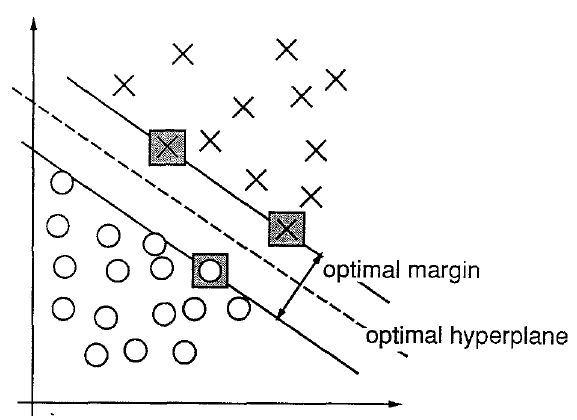
\includegraphics[width=0.5\textwidth]{svm.png}
			\caption{Euclidean Imposition of data. The support vectors, marked with grey squares, define the margin of largest separation between the two classes. \textit{Source: Cortes and Vapnik (1995)} \cite{SVM_cortes1995support}}
		\end{figure}
		
		A key element for SVM statistical and computational power is the \textit{Kernel-Trick} \cite{guyon1993automatic}. The basic problem-formulation in itself seems to present a solution to a very limited spectrum of classification problems, two-dimensional and linearly-separable ones. Using the Kernel-Trick, the linearly dimensional training observations are extrapolated onto a higher plane, with the assumption that on the new plane a better linear separating hyper plane can be found. The extrapolation is carried out using the \textit{trick}, where by the internal product of the linear separator is replaced with a Kernel Function. This Function simulates the redistribution of the original Support Vectors in a richer space, barely incurring an additional computational cost in the process. The linear separator in the new space is not linear on the original plane, thus the classification of new observation is also done using the Kernel Function.
		
		The classification model in itself is natively used for binary classification, therefore 2 classes only. However, as may be the case in many classification scenarios, data has more then 2 dimensions. For the purpose of Multiclass classification using SVMs, a process known as \textit{class-reduction} is implemented \cite{aly2005survey}. This is done by either a 'one-vs-all' or 'one-vs-one' approach. In the former method classifiers for each given class is trained on the entire dataset, and the highest scoring one determines the class for each observation. This is also known as the \textit{winner-takes-all} approach. The latter method consists of a max-wins voting strategy, whereby every observations is denoted to one of two classes by each classifier. The final classification is thereafter determined by a tally of the votes.
		
		Current research of SVM usage revolves around the concept of \textit{Soft-Margins}. In the case of not linearly separable data, which is usually the case, a \textit{hinge loss} function is added to formula. Its purpose is to penalize for observations, which are on the 'wrong' side of the margin, between the 'sidewalk' and 'separator' that is. A trade-off between margin width and the amount of misclassified observations.
		
		Among the advantages of SVMs one can mentions several factors. Firstly, the usage of different kernel - especially user-specified ones, allow for expert knowledge to be integrated into the classification problem. Secondly, the optimization space for the classification problem is convex, thus making it easily solvable with appropriate solving algorithms. And thirdly, the usage of soft-margins, or penalizing for error in classification makes the user more aware of the imminent over-fitting, which is the bane of classification problems. This awareness causes the user to take a more cautious approach. The disadvantages include but are not limited to the following. The choice of kernel is left to decide for the user, which could add to the element of human error, especially with dilettante users. Furthermore, the problem of Multiclass classification is not solved directly, but rather is adopted for, making it not the most effective tool for these cases.
		
		-Strengths and weaknesses\\
		-Math notation\\
		-Sources: \cite{SVM_burges1998tutorial} \cite{SVM_cortes1995support}
	
	\paragraph{Linear Kernel}
	{\color{red}placeholder}
	\paragraph{Polynomial Kernel}
	{\color{red} placeholder}
	\paragraph{Radial Basis Function Kernel}
	{\color{red} placeholder}
	\paragraph{Sigmoid Kernel}
	{\color{red} placeholder}
	
	\subsection*{Neural Networks}
	{\color{red} placeholder} \cite{bishop1995neural}
	\subsection*{Stochastic Gradient Descent}
	{\color{red} placeholder}
	\subsection*{Nearest Neighbors}
	{\color{red} placeholder} \cite{bay1998combining}
	\subsection*{Naive Bayes}
	{\color{red} placeholder} \cite{rish2001empirical}
	\subsection*{Decision Trees and Ensemble Methods}
	{\color{red} placeholder}
	\cite{quinlan2014c4} \cite{breiman1984classification}
	\subsection*{Stochastic Gradient Descent}
	{\color{red} placeholder}
	
	\newpage
	\subsection{Unsupervised Learning}
	{\color{red} placeholder}
	\subsubsection*{Gaussian Mixture}
	{\color{red} placeholder}
	\subsubsection*{Clustering}
	{\color{red} placeholder}
	\subsubsection*{Covariance estimation}
	{\color{red} placeholder}
	\subsubsection*{Neural network models (unsupervised)}
	{\color{red} placeholder}
	
	
	
	
	
	
	
	
	
	
	
	
		
	